te\chapter{Kern der Arbeit}

\anno{ca. 15-20 Seiten}

% Probleme und die Loesungsansaetze
\section{Probleme}
\label{sec:Probleme}

Der im vorherigen Kapitel betrachtete zeitliche Rahmen, über die Entwicklung von Web Application Firewalls, umfasst mehr als zwanzig Jahre. Ein Zeitraum in dem sich zahlreiche Produkte in diesem Bereich etablierten. Im Anhang finden Sie, beispielsweise, unter \ref{tab:my_wafwoof} eine (nicht vollständige) Liste von derzeitigen WAF-Produkten verschiedener Hersteller. Über den gesamten Zeitraum haben sich Webtechnologien weiterentwickelt und auch die Art und Weise der Nutzungs des Internets änderte sich. Mit der Verbreitung der Smartphones und Sprachassistenten wurden aus einfachen Webangeboten vielschichtige Anwendungen mit verschiedenen möglichen Clientsystemen (\emph{mobile-first-Ansatz}). Serviceorientierte Architekturen, Webservices, Microservices, Künstliche Intelligenz - alles entwickelte sich weiter. Im Bereich der IT-Sicherheit veröffentlichte das \emph{Open Web Application Security Project} 2019 erstmals eine Liste seiner zehn kritischsten Sicherheitsrisiken explizit für den Bereich der \emph{API}s. \emph{ModSecurity} ist immernoch der defacto-Standart für regelbasierte WAFs und praktisch so gut wie der einzige verbliebene Vertreter der Web Application Firewalls aus dem OpenSource-Bereich. Freie anomaliebasierte Systeme sind so gut wie nicht existent und die privatwirtschaftlichen Akteure lassen sich kaum in die Karten schauen. \\
Mittlerweile sind bereits dreizehn Jahre seit dem Erscheinen des Datensatzes CSIC2010 vergangen und schaut man in die derzeitig vorhandene Literatur scheint auch kein Nachfolger in Sicht. \\\\

\textcolor{bhtGray}{\ding{110} Applebaum über den Datensatz CSIC2010~\cite{Applebaum2021}} Gimenéz et al. provide an HTTP dataset intended to be used for the development and testing of Intrusion Detections Systems and WAFs. ... The dataset has been used extensively by other researchers ... There is still a need for a development of a new dataset as previous datasets had become outdated and did not target real systems. The dataset .. is itself now over 10 years old and targets a bespoke e-commerce system. \\\\

Dennoch ist der Datensatz weiterhin Ausgangsbasis für viele Forschungsvorhaben und praktische Projekte im Bereich der IT-Sicherheit. Im folgenden Kapitel wird daher näher auf den Datensatz CSIC 2010 eingegangen, dessen Aufbau und Verwendung erläutert und es werden mögliche Verbesserungen anhand von praktischen Beispielen vorgeschlagen.
%

\subsection{Aufbau und Format des Datensatzes CSIC2010}

% Aufbau /motivation von gimenez

% Aufbau
Der Datensatz besteht aus drei Teildatensätzen. Der erste Teildatensatz ist dabei für die Trainingsphase gedacht und enthält 36000 einzelne HTTP-Anfragen die den normalen bzw. erwünschten Datenverkehr abbilden. Die anderen beiden Teildatensätze sind für die Testphase gedacht. Ein Teildatensatz mit ebenfalls 36000 Anfragen an normalem Datenverkehr und ein Teildatensatz mit über 25000 Anfragen mit Gefährdungspotential (siehe \cite{csic2010}).\\

Die einzelnen Dateneinträge der drei Teildatensätze sind jeweils gleich aufgebaut und beinhalten die in Tabelle~\ref{tab:csicfields} aufgeführten Felder. Das Feld \emph{Payload} ist im Datensatz nicht explizit benannt bzw. auf den ersten Blick nicht ersichtlich, da es je nach HTTP-Methode in den Rohdaten unterschiedlich abgebildet wird. Bei einem \verb=GET=-Request wird die Payload im Query der URL übertragen (siehe \cite{rfc2626} 3.2.2) und bei \verb=POST=-Requests im Request Body. Die Payload enthält im Wesentlichen die eigentlichen Daten und in den meisten Angriffsfällen genau die Anomalien die für einen Angriff verantwortlich sind. Zur Verdeutlichung zeigt Abbildung~\ref{fig:ccex} einen einzelnen Eintrag des Datensatzes \emph{CSIC2010} im Rohformat. Hier handelt es sich um einen \verb=GET=-Request mit den Parametern \emph{id},\emph{nombre}, \emph{precio}, \emph{cantidad} und \emph{B1}. Die einzelnen Dateneinträge des Datensatzes unterscheiden sich jedoch nicht in den übrigen Feldern.\\

Für eine Klassifizierung können bzw. müssen aus den Daten der einzelnen Requests entsprechende Features (\emph{Merkmale~-~individuell messbar}) abgeleitet werden. \emph{Achtung}, Felder und Features sind nicht gleichzusetzen! Torrano-Giménez hat in ihrer Doktorarbeit sowohl Features von Experten benennen lassen \footnote{siehe Anhang Tabelle \ref{tab:tgfeatures}} als auch mittels statistischer Feature-Selection-Mechanismen \emph{extrahiert}. Bei den hier vorgeschlagenen Verbesserungen bzw. Änderungen wird sich nur auf die Datenfelder oder auf die benannten \emph{Experten-Features} bezogen.


%\lstset{language=XML,
% 	basicstyle=\ttfamily\color{black}\small,
% 	keywordstyle=\bfseries\color{bhtBlue},
% 	identifierstyle=\color{black}, 
% 	commentstyle=\color{gray}\textsl
% }
\begin{figure}[h]
  \centering
        \caption{Dateneintrag CSIC 2010 Normal Traffic Test}
        \label{fig:ccex}
        \begin{lstlisting}[basicstyle=\footnotesize]
GET http://localhost:8080/tienda1/publico/anadir.jsp
                ?id=1&nombre=Jam%F3n+Ib%E9rico&precio=39&cantidad=41
                &B1=A%F1adir+al+carrito HTTP/1.1
User-Agent: Mozilla/5.0 (compatible; Konqueror/3.5; Linux) KHTML/3.5.8 (like Gecko)
Pragma: no-cache
Cache-control: no-cache
Accept: text/xml,application/xml,application/xhtml+xml,
                text/html;q=0.9;text/plain;q=0.8,image/png,*/*;q=0.5
Accept-Encoding: x-gzip, x-deflate, gzip, deflate
Accept-Charset: utf-8, utf-8;q=0.5, *;q=0.5
Accept-Language: en
Host: localhost:8080
Cookie: JSESSIONID=54E25FF4B7F0E4E855B112F882E9EEa5
Connection: close
\end{lstlisting}
\end{figure}

\begin{sidewaystable}[h]
  \centering
%  \resizebox{\textwidth}{!}{ 
  \begin{tabular}{|l | l | l | l | l | l |}
    \hline
    \textbf{Name} & \textbf{Wert} & \textbf{Anmerkungen} & \textbf{DN} & \textbf{DNT} & \textbf{DNA} \\
    \hline
    HTTP Methode & \verb=GET= oder \verb=POST= im Anomalieteil auch \verb=PUT= & & 2 (0\%) & 2 (0\%) & 3 (0\%)\\
    URL & & & 28 (0\%) & 28 (0\%) & 1623 (0\%)\\
    Protocol & \verb=HTTP/1.1= & HTTP/2 & 1 (0\%) & 1 (0\%) & 1 (0\%)\\
    User-Agent & \verb=Mozilla/5.0 (compatible;Konqueror/3.5...= & & 1 (0\%) & 1 (0\%) & 1 (0\%)\\
    \emph{Pragma} & \verb=no-cache= & & 1 (0\%) & 1 (0\%) & 1 (0\%)\\
    \emph{Cache-control} & \verb=no-cache= & & 1 (0\%) & 1 (0\%) & 1 (0\%)\\
    \emph{Accept} & \verb=text/xml,application/xml,...= & & 1 (0\%) & 1 (0\%) & 1 (0\%)\\
    \emph{Accept-Encoding} & \verb=x-gzip,x-deflate,gzip,deflate= & & 1 (0\%) & 1 (0\%) & 1 (0\%)\\
    \emph{Accept-Charset} & \verb!utf-8,utf-8;q=0.5,*;q=0.5! & & 1 (0\%) & 1 (0\%) & 1 (0\%)\\
    \emph{Accept-Language} & \verb=en= & & 1 (0\%) & 1 (0\%) & 1 (0\%)\\
    Host & \verb=localhost:8080= & & 1 (0\%) & 1 (0\%) & 2 (0\%)\\
    Cookie & \verb=JSESSIONID= verschiedene Werte &  & 36000 (0\%) & 36000 (0\%) & 25065 (0\%) \\
    Content-Type & \verb=null= oder \verb=application/x-www-from-urlencoded= & & 2 (0\%) & 2 (0\%) & 2 (0\%)\\
    \emph{Connection} & \verb=close= & & 1 (0\%) & 1 (0\%) & 1 (0\%)\\
    Content-Length & & & 117 (0\%) & 117 (0\%) & 382 (0\%)\\
    Payload & & & 19418 (0\%) & 20105 (19\%) & 14681 (5\%)\\
    \hline
      % \end{tabular}}
    \end{tabular}
  \caption{Felder des CSIC2010 Datensatzes}
  \label{tab:csicfields}
\end{sidewaystable}

% Format des Datenssatzes Text -> CSV (Referenz zu Dr....) -> ARFF ?? ggf. mit Korrektur

Im Bereich der Anomalie-Requests sieht es ähnlich aus, jedoch wurde hier mit \verb=PUT= noch eine weitere HTTP-Methode angewandt~\cite{csic2010}. \anno{Überleitung}

\subsection{Alter des Datensatzes}

\subsubsection{Das HTTP-Protokoll}

%% Erweiterung HTTP
\subsubsection{Neue Anwendungsarchitekturen}
%% Änderungen Anwendungsarchitekturen


Gwt Verweis\cite{kozik2019}
% SChönes Beispiel für Fortschritt, produktiven Einsatz und zeitliche Veränderung und wo Gimenez nicht funktioniert-- > PUT als anomalie in CSIC2010 definiert aber in REST durchaus üblich
% rest beispiel mit PUT

\begin{figure}[h]
  %% \begin{center}
  \centering
  \includesvg[inkscapelatex=false,width=0.7\textwidth]{Ajax-vergleich}
  \caption{Das Modell einer traditionellen Web-Anwendung (links) im direkten Vergleich mit einer Ajax Web-Anwendung (rechts)~\url{https://commons.wikimedia.org/wiki/File:Ajax-vergleich.svg}}
  \label{fig.ajax}
%%  \end{center}
\end{figure}

\anno{SVG Darstellung korrekt?}


%\lstset{language=XML,
% 	basicstyle=\ttfamily\color{black}\small,
% 	keywordstyle=\bfseries\color{bhtBlue},
% 	identifierstyle=\color{black}, 
% 	commentstyle=\color{gray}\textsl
%      }
\begin{figure}[h]
  \caption{Beispiel für einfachen REST-Request}
  \label{fig:restputexample}
  \begin{lstlisting}
PUT /user/devtty HTTP/1.1
Host: petstore.devtty.de
Content-Type: application/json

{
  "id": 2334,
  "username": devtty,
  "firstName": "Denis",
  "lastName": "Renning"
}
\end{lstlisting}
\end{figure}


\subsubsection{Neue Werkzeuge}

Grundsätzlich sollte auch bedacht werden dass, seit der Erstellung des Datensatzes von Giménez, die genutzten Werkzeuge ebenfalls weiterentwickelt wurden und verbesserte Versionen erschienen. Zum Beispiel wurden zur Erzeugung der Anomalie-Requests die Werkzeuge \emph{Paros}\footnote{\url{https://sourceforge.net/projects/paros/} abgerufen am 29.06.2023} und \emph{w3af}\footnote{\url{https://w3af.org} abgerufen am 29.06.2023} eingesetzt. Die Entwicklung des eigentlichen Paros-Proxies wurde 2006 eingestellt, jedoch übernahm das \emph{Open Web Application Security Project} die Quellen und entwickelte einen Fork der Software unter dem Namen \emph{Zed Attack Proxy}~(ZAP) bis heute weiter. Höchstwahrscheinlich wäre der Umfang der Anomaliedaten wesentlich höher wenn der damalige Testaufbau (mit den aktuelleren Versionen der Software) wiederholt wird und der Generierungsprozess nochmals angestossen wird.
  
\subsection{Ziel des Datensatzes}

Ein weiterer Kritikpunkt Applebaums am Datensatz CSIC2010, neben dem Alter, betrifft das zur Erstellung genutzte Ziel. Für CSIC2010 wurde nur eine einzelne Webanwendung genutzt, die intern vom CSIC2010-Team entwickelt wurde und rudimentäre Funktionen eines e-Commerce-Systems anbietet~\cite{csic2010}. Es existieren eine Nutzerregistrierung und diverse Funktionen aus dem Einkaufsbereich (z.B. Waren einem Einkaufskorb hinzufügen usw.). Applebaum merkt zusätzlich an dass es sich nicht um ein real verwendetes System handelt. Damit beschränken sich die erstellten Daten nur auf den engen Bereich dieser (einen) Webanwendung. 

Erhöhung der allgemeinen Gültigkeit (Diskrepanz mit spezieller Zuschneidung auf Anwendung)~\ref{sec:Probleme}
Erhöhung der Genauigkeit



% Methodik und Vorgehen
\section{Methodik}

% Uebersicht Architektur

\section{Lösungen}

\subsection{Aus Alt mach Neu}

% Hier beschreiben wie CSIC2010 mit "neuen Mitteln" nachgestellt werden kann; warum das nicht geht (fehlende Webanwendung)... ggf. Ersatzanwendung bzw. Übernahme der Originaldatensätze mit in neuen Datensatz

\subsection{Von der Einzelanwendung zur Mehrgültigkeitxxx}

% Hier beschreiben wie durch Verwendung von Demo und Vulnerable-Anwendung mehrgültigkeit geschaffen werden kann
% und Anwendungen nach gleichem Prinzip arbeiten (Entwickler sich ein Beispiel nehmen usw.)


\subsection{Unzureichende Kategorisierung im Datensatz}
% Problem zu viele Falsch-Positive/Zuordnung:Framework/Status(Session) -> Anwendungsstatus (DeltaspikeClientId/SpringExecuteID)
% möglichkeit anomalien nicht auf basis der Regeln sondern auf basis von abweichungen in der Anwendungsnutzung auszuwerten

% Erweiterung Datenset um Variablen (eingeloggt/framework/id)
% Notwendigkeit auf gegeben das CTGimenez Datensatz auf einer Anwendung basierte und nur gegen diese getestet wurde -> Testen gegen andere Anwendung aber gleicher Art?


\subsection{Zentralisierung}

\begin{figure}[ht]
  \begin{center}
    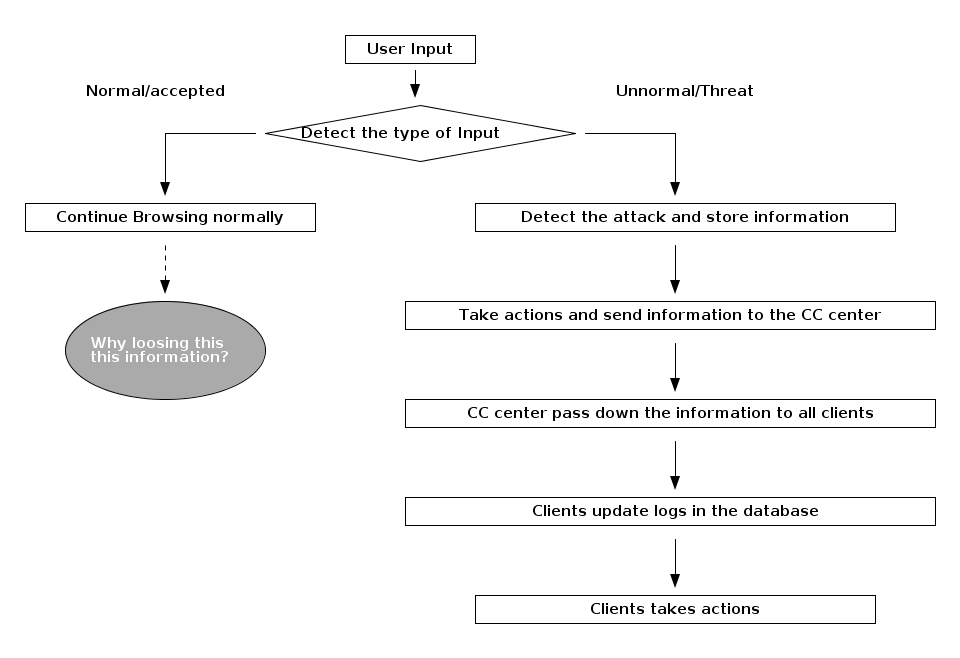
\includegraphics[width=15cm]{waf_mana}
    \caption{Zentralisiert~\cite{Manaseer2018}}
    \label{fig.topten}
  \end{center}
\end{figure}

% Oder: Der xxx Algorithmus

% Oder: Der yyy Algorithmus

% Zusammenfassung: ca. 0,5 Seiten
\section{Zusammenfassung}

Nach der kurzen zeitlichen Einordnung über die Entstehung anomaliebasierter Web Application Firewalls im vorherigen Kapitel lieferte dieses Kapitel einen Einblick in einen Teil der bestehenden Daten. Dazu wurde der Umfang und Inhalt des2010 von Carmen Torrano-Giménez erstellten Datensatzes \emph{CSIC2010} näher betrachtet. Es wurden einige Modernisierungsmaßnahmen vorgeschlagen, die dem veralteten Datensatz zu etwas mehr Allgemeingültigkeit und vor allem Genauigkeit verhelfen.

Das nächste Kapitel betrachtet die praktische Umsetzung der angedachten Ziele. Es soll dargestellt werden, wie ein neuer Datensatz generiert bzw. der bestehende Daten erweitert werden und wie neue Daten gesammelt werden können. 

\begin{neu}
  Anfang mit Aufnahme des Altenbestands, hinzufügen Entwicklungsumgebung, Test, etc

  Entwicklung Zentrale Steuerung

  Entwicklung ML Anteil
\end{neu}